\documentclass{article}

% This is for figures.
\usepackage{graphicx}

% This is for comments/verbatim content.
\usepackage{comment}

% This is for references.
\usepackage{natbib} \bibpunct[,]{(}{)}{;}{a}{,}{,}

% This is for hyperlinks.
\usepackage{hyperref}

% Rather than including the relative path for each figure, you can set a path
% to be searched here. Make sure all figures have distinctive names otherwise
% you may end up having different plots than you were expecting.
\graphicspath{{figures_tables/}}


\title{Paper 1 title}
\author{Paper 1 authors}


% Often more content will exist in your thesis than ends up in the final 
% manuscript. This environment will allow you to include content in the thesis
% that is not included in the manuscript.
\newenvironment{thesis}{}{}
\excludecomment{thesis} % will exclude material that is only for the thesis


\begin{document}


\maketitle

\section{Introduction}
Put chapter 1 content here.

\begin{thesis}
Wrap content you only want for the thesis using the thesis environment.  
This content will be included in the thesis, 
but not in the submitted/published version of the manuscript.
\end{thesis}

\section{Lets make a table} 
% latex table generated in R 3.3.0 by xtable 1.8-2 package
% Thu May 18 10:23:23 2017
\begin{table}[ht]
\centering
\caption{Captions go above tables.} 
\label{t1}
\begin{tabular}{rrrrr}
  \hline
 & X1 & X2 & X3 & X4 \\ 
  \hline
1 &   9 &   8 &  14 &  13 \\ 
  2 &   7 &  11 &   9 &  11 \\ 
  3 &   8 &   6 &  10 &   9 \\ 
  4 &   6 &  10 &  11 &  16 \\ 
   \hline
\end{tabular}
\end{table}
 

\section{Figures}

\subsection{Lets share an historic moment}

Figure \ref{history} is so amazing  that the rest is indeed obvious.
\begin{figure}[h!tb] \centering
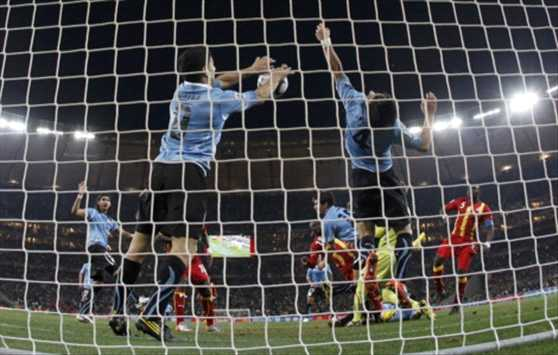
\includegraphics{history}
\caption{Suarez save the day !}
\label{history}
\end{figure}
Captions go beneath figures.

\section{References}

For references, use BibTeX (\url{http://www.bibtex.org/}).
This means you will want a file that includes your references, 
e.g. references.bib, and you will reference them using a set of BibTeX commands.

\cite{niemi2015empirical} constructed a hierachical model and an empirical 
Bayes analysis for RNA-seq data. 
An analysis of RNA-seq data showed large number of genes exhibiting a pattern
of hybrid vigor \citep{niemi2015empirical}.
\citeauthor{niemi2015empirical} can be extended for many different experimental
designs.


% For references
\bibliography{references}    % file with .bib extension containing your references
\bibliographystyle{plainnat} % style of bibliography

\end{document}

